\documentclass[12pt]{article}
\usepackage{../lp,graphicx,amsmath}
\usepackage{tkz-berge}
% Cross-references for handout numbers.
\usepackage{amsfonts}
%\usepackage{amsthm}
\usepackage{hyperref}
\usepackage{amssymb}
%\usepackage[capitalize]{cleveref}
\usepackage{xcolor}

%\input{handouts}

\newcounter{chapnum}

\newtheorem{definition}{Definition}[chapnum]
\newtheorem{remark}{Remark}[chapnum]
\newtheorem{theorem}{Theorem}[chapnum]
\newtheorem{lemma}[theorem]{Lemma}
\newtheorem{corollary}[theorem]{Corollary}
\newtheorem{proposition}[theorem]{Proposition}
\newtheorem{claim}[theorem]{Claim}
\newtheorem{observation}{Observation}[chapnum]

\renewcommand{\thesection}{\arabic{chapnum}.\arabic{section}}
\renewcommand{\thefigure}{\arabic{chapnum}.\arabic{figure}}


\newenvironment{proof}{\noindent{\bf Proof:} \hspace*{1em}}{
        \hspace*{\fill} $\triangle$ }
\newenvironment{proof_of}[1]{\noindent {\bf Proof of #1:}
        \hspace*{1em} }{\hspace*{\fill} $\triangle$ }
\newenvironment{proof_claim}{\begin{quotation} \noindent}{
        \hspace*{\fill} $\diamond$ \end{quotation}}
\newenvironment{solution}{\noindent{\bf Solution:} \hspace*{1em}}{
        \hspace*{\fill} $\triangle$ }


\newcommand{\R}{{\mathbb R}}
\newcommand{\Z}{{\mathbb Z}}
\newcommand{\Q}{{\mathbb Q}}
\newcommand{\C}{{\mathbb C}}
\newcommand{\N}{{\mathbb N}}
\newcommand{\lin}{\operatorname{lin}}
\newcommand{\aff}{\operatorname{aff}}
\newcommand{\cone}{\operatorname{cone}}
\newcommand{\conv}{\operatorname{conv}}
\newcommand{\vol}{\operatorname{vol}}
\newcommand{\poly}{\operatorname{poly}}




\newcommand{\CF}[1]{{\color{purple}[CF: #1]}}


\newlength{\toppush}
\setlength{\toppush}{2\headheight}
\addtolength{\toppush}{\headsep}

\newcommand{\htitle}[2]{\noindent\vspace*{-\toppush}\newline\parbox{6.5in}
{Massachusetts Institute of Technology \hfill 18.453: Combinatorial Optimization 
\newline
\textbf{Instructor:} Cole Franks \quad \textbf{Notes: }Michel Goemans and Zeb Brady \hfill#2\newline
\mbox{}\hrulefill\mbox{}}\vspace*{1ex}\mbox{}\newline
\begin{center}{\Large\bf #1}\end{center}}

\newcommand{\handout}[2]{\thispagestyle{empty}
 \markboth{ #1 \hfil #2}{ #1 \hfil #2}
 \pagestyle{myheadings}\htitle{#1}{#2}}


\setlength{\oddsidemargin}{0pt}
\setlength{\evensidemargin}{0pt}
\setlength{\textwidth}{6.5in}
\setlength{\topmargin}{0in}
\setlength{\textheight}{8.5in}


\newcounter{exercisenum}
\newcounter{exercisetot}
\setcounter{exercisetot}{0}



\newenvironment{exercises}{
	\begin{list}{{\bf Exercise \arabic{chapnum}-\arabic{exercisenum}. \hspace*{0.5em}}}
	{\setlength{\leftmargin}{0em}
	 \setlength{\rightmargin}{0em}
	 \setlength{\labelwidth}{0em}
	 \setlength{\labelsep}{0em}
	\usecounter{exercisenum}
      \setcounter{exercisenum}{\theexercisetot}}}{\setcounter{exercisetot}{\theexercisenum}\end{list}}


\newenvironment{pseudocode}{
    \begin{list}{}{
        \renewcommand{\makelabel}{$\triangleright$}
        \setlength{\topsep}{0pt}
        \setlength{\leftmargin}{32pt}
        \setlength{\labelwidth}{14pt}
        \setlength{\labelsep}{0mm}
        \setlength{\itemindent}{0mm}
        \setlength{\itemsep}{-3pt}
        \setlength{\itemsep}{0mm}
        \setlength{\parsep}{0pt}%
        \setlength{\listparindent}{0pt}
    }
}
{
    \end{list}
}

\newcommand{\rank}{\operatorname{rank}}

\setlength{\topmargin}{-1in}
\setlength{\textheight}{9.7in}
%\usepackage{epsfig}
\begin{document}

%\handout{QUIZ 1}{April 11th, 2017}

\noindent {\Large 18.453 Quiz, Spring 2021} \\
~\\

\paragraph{Instructions.} This is a {\bf timed} quiz. Turn this quiz by submitting a pdf or image to gradescope at most \textbf{2} hours after opening it. You may use notes and course material, but collaboration is not allowed. You may quote anything stated in the course material or lecture notes without justification, including exercises (except exercises that appear in the quiz itself). Questions are worth 4 points unless otherwise mentioned.

\textbf{Failure to adhere to these rules may result in a grade of zero for the assignment, and referral to the Committee on Discipline.}
%For best practice I suggest trying to complete it under these conditions. Afterwards please tell me if 2 hours felt like enough. 
%Please write the solutions as neatly as possible and show your steps. Your grade will be the average of these two grades. 


\begin{enumerate}
\item Find a minimum vertex cover in the following
graph, and give a short argument for its optimality. 

%\begin{center}
%\includegraphics{mat1}
%\end{center}

%vertex cover: a0, a1, b1, a3
%matching: a0b0, a1b2, a3b3, a4b1
\begin{center}
\begin{tikzpicture}
   \begin{scope}[rotate=90]
       \SetVertexMath
       \grEmptyLadder[RA=-2,RB=-4]{5}   
   \end{scope}
    \Edges(a0,b0,a1,b2,a3,b3,a1)
    \Edges(a4,b1)
    \Edges(b1,a2)
    \Edges(a1,b4,a3)
    \Edges(b1,a0,b2)
\end{tikzpicture}
\end{center}
%%%%%%%%%%%%%%%%%
\newpage
Blank page 
\newpage

\item 
Let $U$ be any minimizer in the Tutte-Berge formula. Let $K_1,
  \cdots, K_k$ be the connected components of $G\setminus U$.  
  
Show
  that, for {\it any} maximum matching $M$, we must have that $M$ contains exactly $\lfloor \frac{|K_i|}{2}\rfloor$ edges from
$G[K_i]$ (the subgraph of $G$ induced by the vertices in
$K_i$).\footnote{ i.e. $G[K_i]$ is perfectly matched for the even components $K_i$ and
near-perfectly matched for the odd components. }
%\begin{enumerate}
%\item
%\item Each vertex $u\in U$ is matched to a vertex $v$ in an odd component $K_i$ of $G\setminus U$.
%\item the only unmatched vertices must be in odd components $K_i$ of $G\setminus U$.  
%\end{enumerate}  
\newpage
Blank page
\newpage
%%%%%%%%%%%%%%%%%%

\item 
\begin{enumerate}
\item Do there exist three points in $\R^2$ that are affinely independent? If so, draw an example.
\item Do there exist two points in $\R^2$ that are affinely independent but linearly \emph{dependent}? If so, draw an example.
\item Draw the linear hull $\lin(S)$, affine hull $\aff(S)$, conic hull $\cone(S)$, and convex hull $\conv(S)$ of the set of points 
$$S  = \{(0,1), (2,1), (1,3), (1,2) \} \subset \R^2,$$
and give a description of each in the form $\{x: Ax \leq b\}$.\footnote{If the set you are trying to describe is equal to all of $\R^2$, i.e. has no inequalities, just write that it is equal to $\R^2$.} No justification is needed.
\end{enumerate}

\newpage
Blank page 
\newpage 

\item Let
$$ A = \begin{bmatrix} 
 1 &  1 & 0 & 0 \\ 
 0 & 0 & 1 & 1 \\
 1 & 0 & 1 & 0 
\end{bmatrix}. $$
\begin{enumerate}
\item State the dual of the following LP: \footnote{To avoid confusion, I'll let you know that you do \textbf{not} need the answer from part (a) for part (b).} 
\lps
  &  &  & \mbox{Min} &   (1,2,1,3) \cdot x\\
  & \lefteqn{\mbox{subject to:}} \\
  &        &   &  &   Ax = (2,3,1)^T \\
  &       &   &  & x \geq 0.
\elps
\item Suppose $b$ is in $\Z^3$. Show that either the polyhedron $P = \{x: Ax \leq b, x \geq 0\}$ is empty or all the vertices of $P$ are integral. 
\end{enumerate}
\newpage
Blank page
%\item Show that if $\rank(A)<n$ then $P=\{x\in \R^n: Ax \leq b\}$ has no vertices.
%\newpage

%\item Consider the polyhedron $P = \{x \in \R^n: Ax \leq b, x \geq 0\}$ where $A \in \R^{m\times n}, b \in \R^m$ and every entry of $A$ is in $\{0, -1, +1\}$. Suppose every column of $A$ has either (i) at most one nonzero entry or (ii) exactly two nonzero entries, one of which is $+1$ and the other $-1$. E.g.$$\begin{bmatrix} 0 & 1 & -1 \\ 0 & 0 & 1 \\ 1 & -1 & 0 \end{bmatrix}.$$Show that $P$ is integral, i.e. every vertex of $P$ is in $\Z^m$.\newpage

%%%%%%%%%%%%%
\newpage

\item \textbf{Extra credit: (2 pts)} The incidence matrix of a directed graph $G = (V, E)$ is a $|E| \times |V|$ matrix with a row for each edge $(u,v)$ with a $1$ in the $u$ entry and a $-1$ in the $v$ entry and zeroes elsewhere. For example, the indicence matrix of the directed $3$-cycle $(1,2), (2,3), (3,1)$ is 
$$
A = \begin{bmatrix} 
 1 &  -1 & 0  \\ 
 0 & 1 & -1  \\
 -1 & 0 & 1 
\end{bmatrix}. 
$$
Show that the indidence matrix of a directed graph is totally unimodular. 
\newpage
Blank page
\end{enumerate}







\end{document}
